% Options for packages loaded elsewhere
\PassOptionsToPackage{unicode}{hyperref}
\PassOptionsToPackage{hyphens}{url}
%
\documentclass[
]{book}
\usepackage{amsmath,amssymb}
\usepackage{lmodern}
\usepackage{iftex}
\ifPDFTeX
  \usepackage[T1]{fontenc}
  \usepackage[utf8]{inputenc}
  \usepackage{textcomp} % provide euro and other symbols
\else % if luatex or xetex
  \usepackage{unicode-math}
  \defaultfontfeatures{Scale=MatchLowercase}
  \defaultfontfeatures[\rmfamily]{Ligatures=TeX,Scale=1}
\fi
% Use upquote if available, for straight quotes in verbatim environments
\IfFileExists{upquote.sty}{\usepackage{upquote}}{}
\IfFileExists{microtype.sty}{% use microtype if available
  \usepackage[]{microtype}
  \UseMicrotypeSet[protrusion]{basicmath} % disable protrusion for tt fonts
}{}
\makeatletter
\@ifundefined{KOMAClassName}{% if non-KOMA class
  \IfFileExists{parskip.sty}{%
    \usepackage{parskip}
  }{% else
    \setlength{\parindent}{0pt}
    \setlength{\parskip}{6pt plus 2pt minus 1pt}}
}{% if KOMA class
  \KOMAoptions{parskip=half}}
\makeatother
\usepackage{xcolor}
\usepackage{longtable,booktabs,array}
\usepackage{calc} % for calculating minipage widths
% Correct order of tables after \paragraph or \subparagraph
\usepackage{etoolbox}
\makeatletter
\patchcmd\longtable{\par}{\if@noskipsec\mbox{}\fi\par}{}{}
\makeatother
% Allow footnotes in longtable head/foot
\IfFileExists{footnotehyper.sty}{\usepackage{footnotehyper}}{\usepackage{footnote}}
\makesavenoteenv{longtable}
\usepackage{graphicx}
\makeatletter
\def\maxwidth{\ifdim\Gin@nat@width>\linewidth\linewidth\else\Gin@nat@width\fi}
\def\maxheight{\ifdim\Gin@nat@height>\textheight\textheight\else\Gin@nat@height\fi}
\makeatother
% Scale images if necessary, so that they will not overflow the page
% margins by default, and it is still possible to overwrite the defaults
% using explicit options in \includegraphics[width, height, ...]{}
\setkeys{Gin}{width=\maxwidth,height=\maxheight,keepaspectratio}
% Set default figure placement to htbp
\makeatletter
\def\fps@figure{htbp}
\makeatother
\setlength{\emergencystretch}{3em} % prevent overfull lines
\providecommand{\tightlist}{%
  \setlength{\itemsep}{0pt}\setlength{\parskip}{0pt}}
\setcounter{secnumdepth}{5}
\usepackage{booktabs}
\ifLuaTeX
  \usepackage{selnolig}  % disable illegal ligatures
\fi
\usepackage[]{natbib}
\bibliographystyle{plainnat}
\IfFileExists{bookmark.sty}{\usepackage{bookmark}}{\usepackage{hyperref}}
\IfFileExists{xurl.sty}{\usepackage{xurl}}{} % add URL line breaks if available
\urlstyle{same} % disable monospaced font for URLs
\hypersetup{
  pdftitle={HemaScope Tutorial},
  pdfauthor={Zhenyi Wang, Yuxin Miao, and Junyi Zhang},
  hidelinks,
  pdfcreator={LaTeX via pandoc}}

\title{HemaScope Tutorial}
\author{Zhenyi Wang, Yuxin Miao, and Junyi Zhang}
\date{2024-07-04}

\begin{document}
\maketitle

{
\setcounter{tocdepth}{1}
\tableofcontents
}
\hypertarget{introduction}{%
\chapter{Introduction}\label{introduction}}

HemaScope is a specialized bioinformatics toolkit designed for analyzing both single-cell and spatial transcriptome sequencing data from hematopoietic cells, including myeloid and lymphoid lineages. We have developed an R package named HemaScopeR, a Shiny interface named HemaScopeShiny, and a cloud platform named HemaScopeCloud.

This tutorial introduces how to install and use the R package and Shiny interface, as well as how to access and operate the cloud platform.

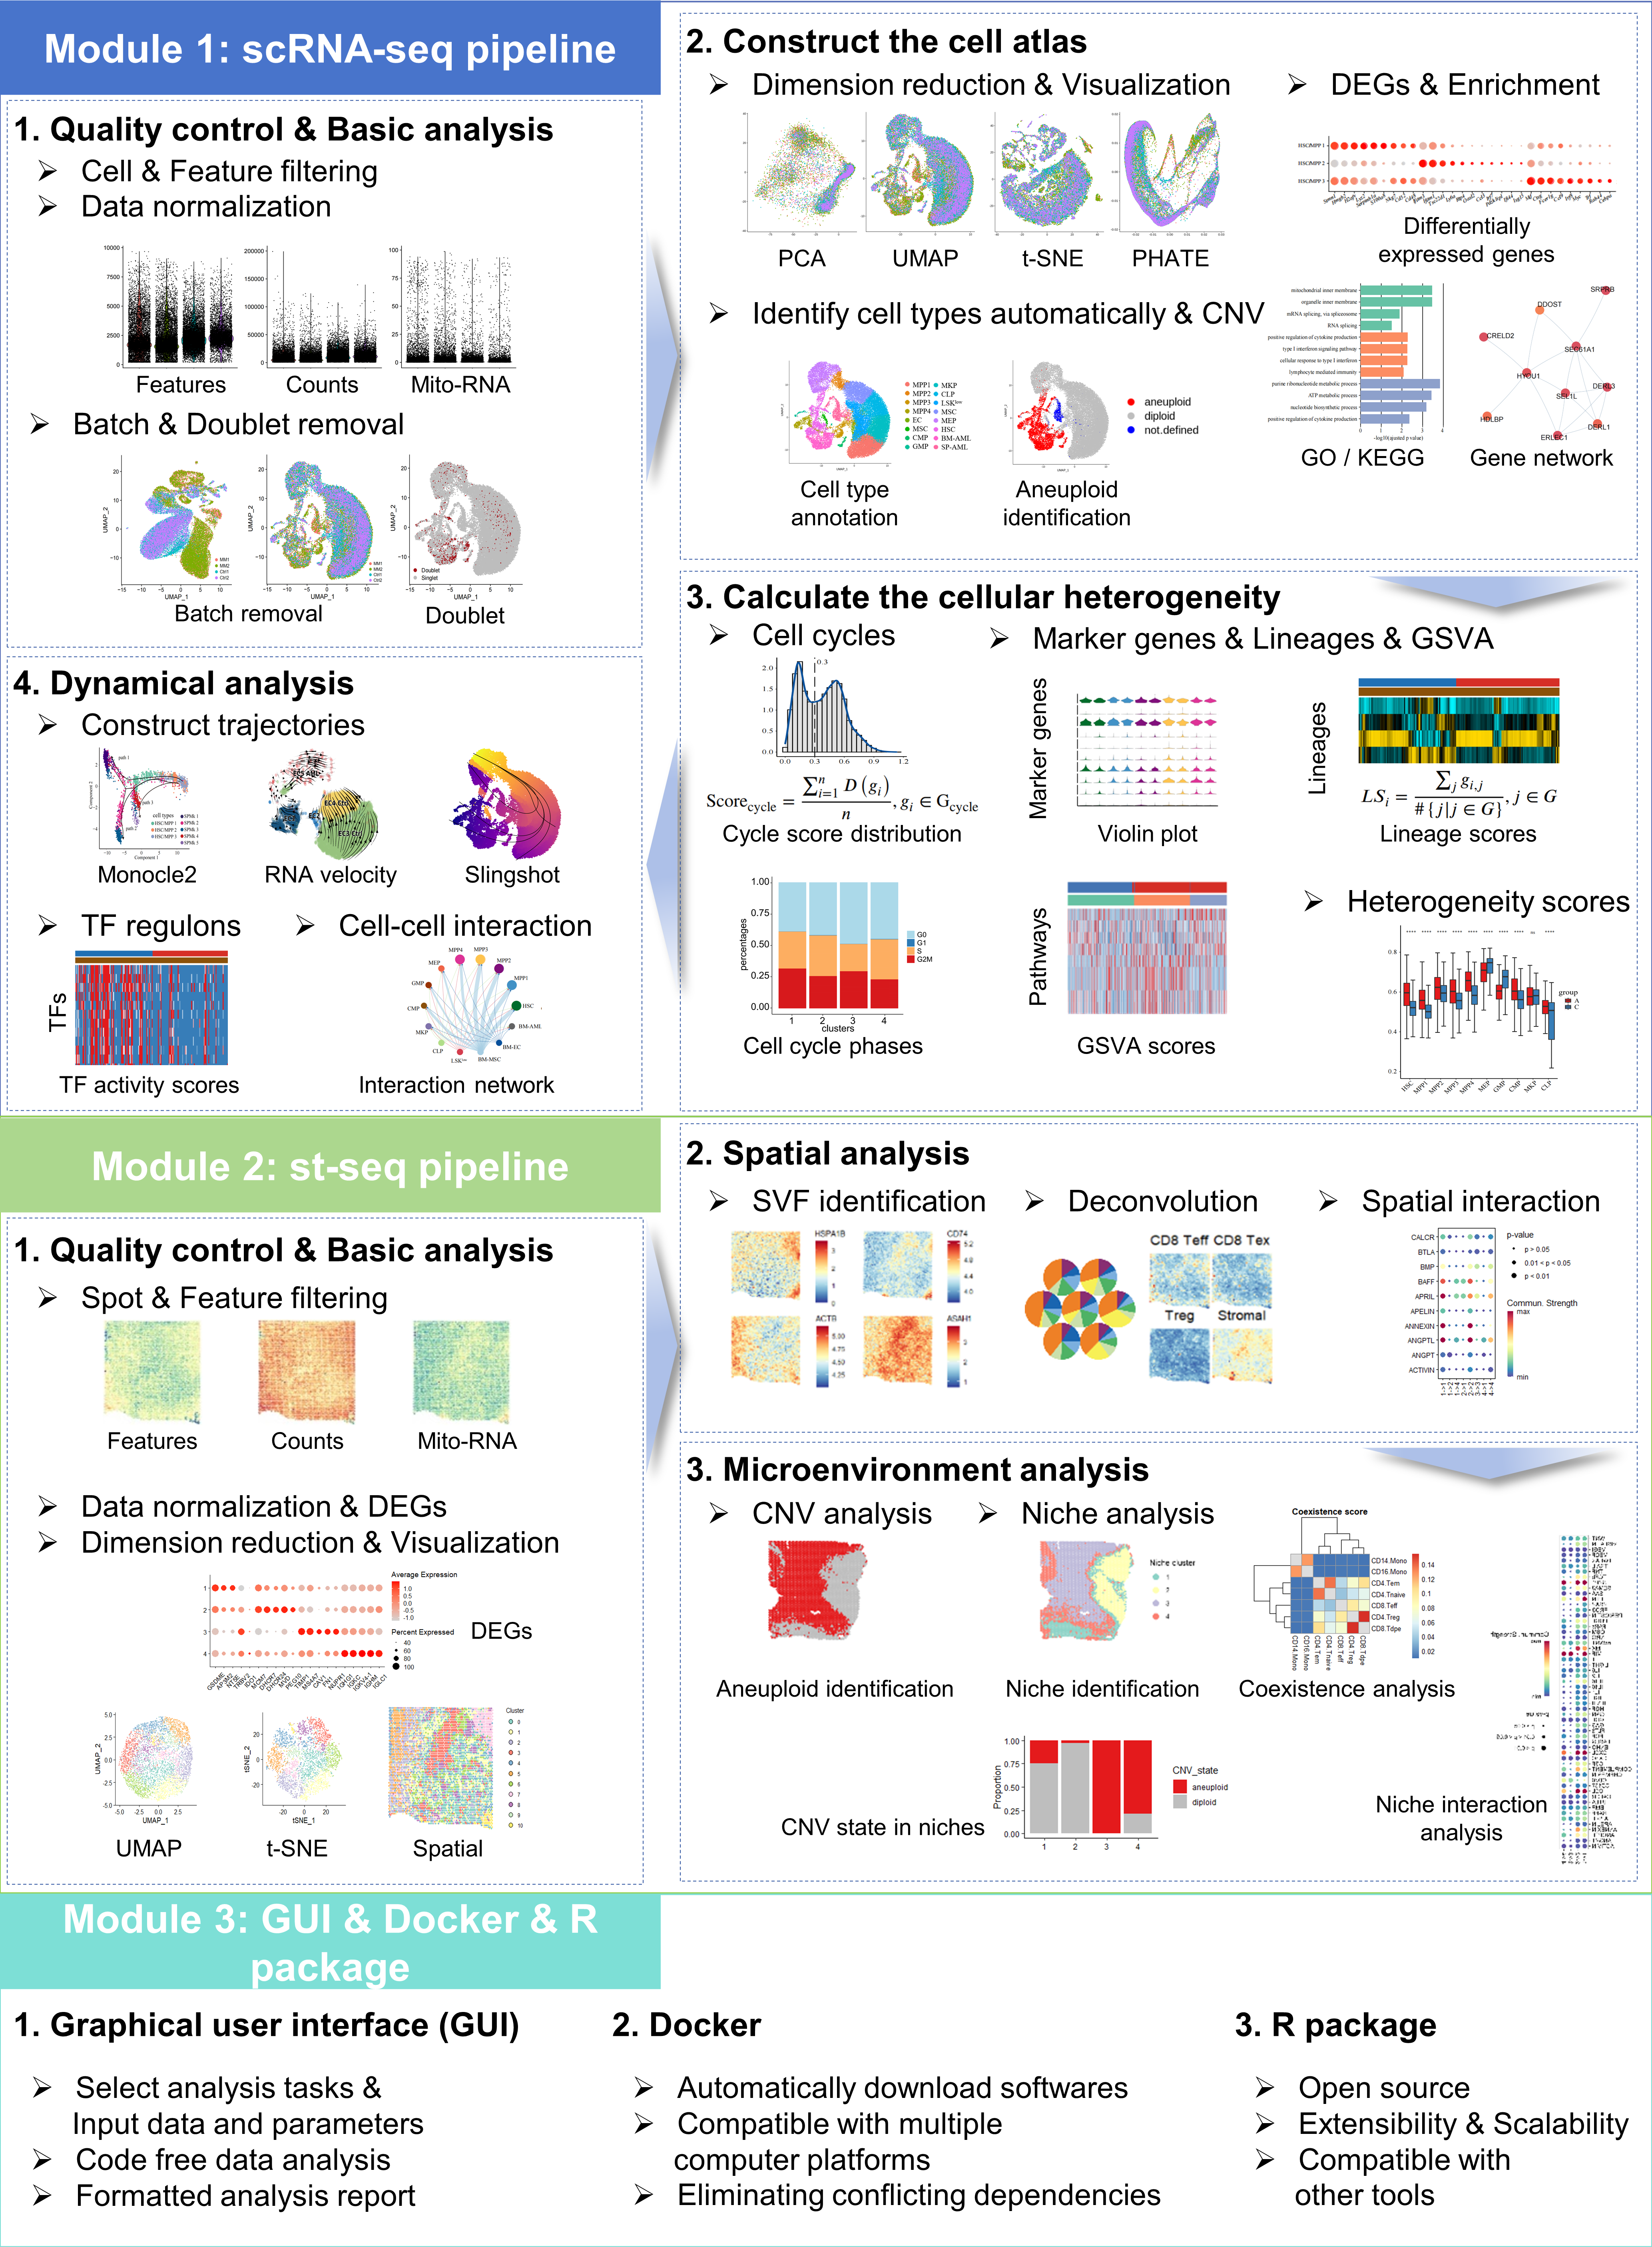
\includegraphics[width=1\linewidth]{images/Figure1_latest}

\hypertarget{installation}{%
\chapter{Installation}\label{installation}}

\hypertarget{install-r-and-python}{%
\section{Install R and python}\label{install-r-and-python}}

\begin{itemize}
\tightlist
\item
  Create a new conda environment,install R 4.3.3 and python 3.11.4
\end{itemize}

\begin{verbatim}
conda create --name HemaScopeR_env
conda activate HemaScopeR_env
conda install R-base=4.3.3
conda install python=3.11.4
\end{verbatim}

\hypertarget{install-required-r-packages}{%
\section{Install required R-packages}\label{install-required-r-packages}}

\begin{itemize}
\tightlist
\item
  install high-priority packages
\end{itemize}

R:

\begin{verbatim}
install.packages("BiocManager",version="1.30.23")
BiocManager::install("ComplexHeatmap",version="2.18.0")     
BiocManager::install("scmap")
\end{verbatim}

Conda:

\begin{verbatim}
 conda config --add channels bioconda
 conda install -c conda-forge r-devtools=2.4.5      
 conda install -c conda-forge r-Seurat=5.1.0        
 conda install -c conda-forge r-Rfast2=0.1.5.1      
 conda install -c conda-forge r-hdf5r=1.14.3
\end{verbatim}

\begin{itemize}
\tightlist
\item
  install required packages from cran
\end{itemize}

\begin{verbatim}
install.packages("shiny", version = "1.8.1.1")
install.packages("textshaping", version = "0.4.0")
install.packages("shinyjs", version = "2.1.0")
install.packages("phateR", version = "1.0.7")
install.packages("plyr", version = "1.8.9")
install.packages("dplyr", version = "1.1.4")
install.packages("ggpubr", version = "0.6.0")
install.packages("viridis", version = "0.6.4")
install.packages("pheatmap", version = "1.0.12")
install.packages("feather", version = "0.3.5")
install.packages("foreach", version = "1.5.2")
install.packages("doParallel", version = "1.0.17")
install.packages("RColorBrewer", version = "1.1-3")
install.packages("gelnet", version = "1.2.1")
install.packages("ggplot2", version = "3.5.1")
install.packages("parallelDist", version = "0.2.6")
install.packages("patchwork", version = "1.2.0")
install.packages("markdown", version = "1.12")
install.packages("kableExtra", version = "1.3.4")
install.packages("transport", version = "0.14-6")
\end{verbatim}

\begin{itemize}
\tightlist
\item
  install required packages from BiocManager(Give every ``Proceed?'' a
  ``y'')
\end{itemize}

\begin{verbatim}
conda install -c bioconda bioconductor-monocle=2.28.0
conda install -c bioconda bioconductor-slingshot=2.8.0
conda install -c bioconda bioconductor-GSVA=1.48.2
conda install -c bioconda bioconductor-limma=3.56.2
conda install -c bioconda bioconductor-org.Mm.eg.db=3.17.0
conda install -c bioconda bioconductor-org.Hs.eg.db=3.17.0
conda install -c bioconda bioconductor-scran=1.24.0
conda install -c bioconda bioconductor-AUCell=1.22.0
conda install -c bioconda bioconductor-RcisTarget=1.20.0
conda install -c bioconda bioconductor-GENIE3=1.24.0
conda install -c bioconda bioconductor-clusterProfiler=4.8.1
conda install -c bioconda bioconductor-biomaRt=2.56.1
\end{verbatim}

\begin{itemize}
\tightlist
\item
  install required packages from GitHub
\end{itemize}

tips:

Sometimes network connection issues may occur, resulting in an error message indicating that GitHub cannot be connected. Please try installing again when the network conditions improve.

Usage limitations: Sometimes an API rate limit error occurs, and a GitHub token is needed to provide the GitHub API rate limit. The steps to resolve this are as follows: Register for an account or log in to an existing account on the GitHub website. Then click on your profile picture in the top right corner, go to the dropdown menu and select ``Settings.'' Next, find ``Developer settings'' and click on it, then find ``Personal access tokens (classic).'' Click on it, then click ``Create new token (classic).'' Create a new token by first naming it anything you like. Then choose the expiration time for the token. Finally, check the ``repo'' box; the token will be used to download code repositories from GitHub. Click ``Generate token.'' Copy the generated token password.

After that, set the token in the environment variable in R. Since we are using conda, enter R by typing R in the terminal. Then, enter the command: usethis::edit\_r\_environ(). This will open a file. Press the i key to edit. Paste the token you copied into the code area as follows: GITHUB\_TOKEN=``your\_token''.

Then press Esc, type :wq! (force save). After that, you need to exit Linux and re-enter R. Close and reopen the terminal to apply the environment variable. Reopen Linux, activate the conda environment, and enter R again.

R:

\begin{verbatim}
devtools::install_github("jinworks/CellChat")
devtools::install_github("aertslab/SCENIC")
devtools::install_github("pzhulab/abcCellmap")
devtools::install_github("navinlabcode/copykat")
remotes::install_github('chris-mcginnis-ucsf/DoubletFinder')
remotes::install_github('satijalab/seurat-wrappers')
remotes::install_github("mojaveazure/seurat-disk")
\end{verbatim}

conda:

\begin{verbatim}
conda install -c bioconda r-velocyto.r=0.6
\end{verbatim}

\begin{itemize}
\tightlist
\item
  Installed R packages with version:
\end{itemize}

\begin{verbatim}
Bioconductor 3.18 
BiocManager 1.30.23
Devtools 2.4.5
Matrix 1.6-5
shiny 1.8.1.1
textshaping 0.4.0
shinyjs 2.1.0
Seurat 5.1.0
phateR 1.0.7
DoubletFinder 2.0.4
monocle 2.28.0
slingshot 2.8.0
GSVA 1.48.2
limma 3.56.2
plyr 1.8.9
dplyr 1.1.4
org.Mm.eg.db 3.17.0
org.Hs.eg.db 3.17.0
CellChat 2.1.2
velocyto.R 0.6
SeuratWrappers 0.3.5
stringr 1.5.1
scran 1.24.0
ggpubr 0.6.0
viridis 0.6.4
pheatmap 1.0.12
parallel 4.3.3
reticulate 1.37.0
SCENIC 1.3.1
feather 0.3.5
AUCell 1.22.0
RcisTarget 1.20.0
foreach 1.5.2
doParallel 1.0.17
clusterProfiler 4.8.1
RColorBrewer 1.1-3
Rfast2 0.1.5.1
SeuratDisk 0.0.0.9020
abcCellmap 0.1.0 
biomaRt 2.56.1
copykat 1.1.0
gelnet 1.2.1
ggplot2 3.5.1
parallelDist 0.2.6
patchwork 1.2.0
markdown 1.12
GENIE3 1.24.0
\end{verbatim}

\hypertarget{install-required-python-packages}{%
\section{Install required Python-packages}\label{install-required-python-packages}}

\begin{itemize}
\tightlist
\item
  upgrade pip and set mirrors
\end{itemize}

\begin{verbatim}
python -m pip install -i https://pypi.tuna.tsinghua.edu.cn/simple --upgrade pip
pip config set global.index-url https://pypi.tuna.tsinghua.edu.cn/simple
pip config set global.extra-index-url http://mirrors.aliyun.com/pypi/simple/
\end{verbatim}

\begin{itemize}
\tightlist
\item
  install required packages
\end{itemize}

\begin{verbatim}
pip install numpy==1.23.5
pip install pandas==2.2.2
pip install matplotlib==3.5.2
pip install scvelo==0.2.5
pip install arboreto==0.1.6
pip install pot==0.9.1
pip install anndata==0.9.2
pip install scanpy==1.9.4
pip install scipy==1.11.2
pip install seaborn==0.12.2
pip install commot==0.0.3
pip install scvi-tools==1.0.3
pip install cell2location==0.1.3 
#import cell2location:2 warnings
pip install phate==1.0.11
pip install jax==0.4.20
pip install jaxlib==0.4.20
\end{verbatim}

\hypertarget{install-hemascoper}{%
\section{Install HemaScopeR}\label{install-hemascoper}}

\begin{verbatim}
devtools::install_github(repo="ZhenyiWangTHU/HemaScopeR", dep = FALSE)
\end{verbatim}

\hypertarget{scrna-seq-pipeline}{%
\chapter{ScRNA-seq Pipeline}\label{scrna-seq-pipeline}}

\hypertarget{step-1.-load-data}{%
\section{Step 1. Load Data}\label{step-1.-load-data}}

This is the step 1 in the scRNA-seq pipeline.

  \bibliography{book.bib,packages.bib}

\end{document}
